\documentclass[10pt,a4paper]{article}
\usepackage[utf8]{inputenc}
\usepackage[margin=18mm]{geometry}
\usepackage{amsmath,amssymb}
\usepackage{graphicx}
\usepackage{booktabs}
\usepackage{tabularx}
\usepackage{hyperref}
\usepackage{microtype}
\usepackage{fancyvrb}
\usepackage[T1]{fontenc}
\usepackage{float}

\hypersetup{colorlinks=true, linkcolor=blue, urlcolor=blue}

\title{\textbf{CS F320 Foundations of Data Science -- Assignment 1}}
\author{}
\date{}

\begin{document}
\maketitle
\vspace{-2em}
\begin{center}
\begin{tabular}{|lr|}
\toprule
Name & ID \\
\midrule
B.N.R. Krishna & 2024A7PS0175H \\
Sudhanva B H & 2024A7PS0085H \\
\bottomrule
\end{tabular}
\end{center}

\noindent\textbf{Setup:} Python with NumPy implemented from scratch (no scikit-learn); random seed 42 for SGD and mini-batch shuffling.

\section{P1 -- Closed Form and the Gradient-Descent Family}

\subsection{D1 -- Closed-Form Fits and Condition Numbers}
\begin{figure}[H]
\centering
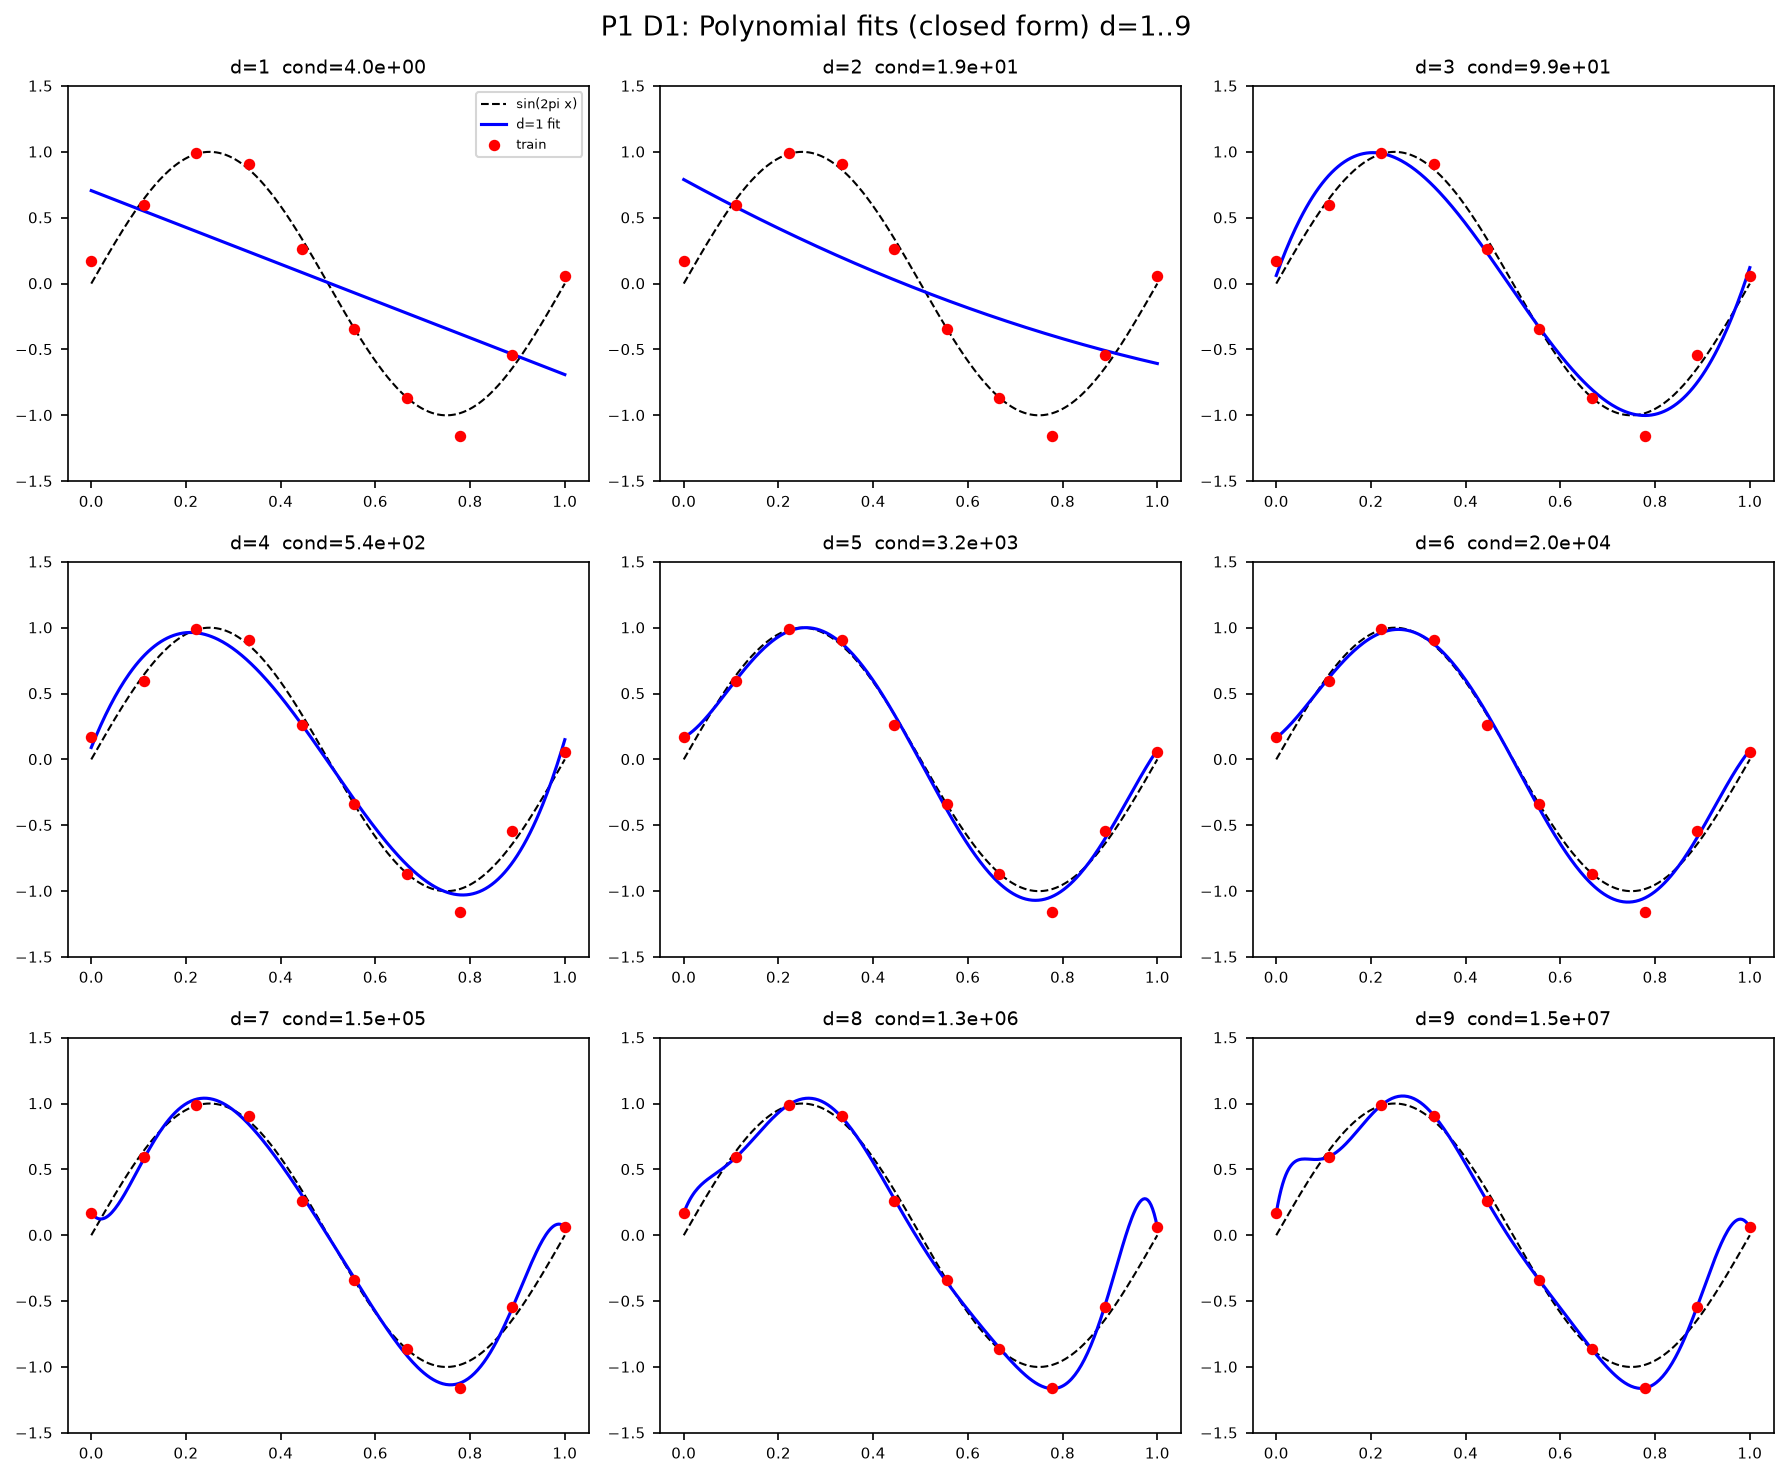
\includegraphics[width=0.88\linewidth]{images/p1_d1_closed_form_fits.png}
\caption{Closed-form polynomial fits, degrees 1–9}
\end{figure}
\begin{table}[H]
\centering
\caption{Condition numbers of Phi vs polynomial degree}
\small
\begin{tabular}{|lr|}
\toprule
Degree & cond(Phi) \\
\midrule
1 & 3.9849e+00 \\
2 & 1.9204e+01 \\
3 & 9.9026e+01 \\
4 & 5.4143e+02 \\
5 & 3.1696e+03 \\
6 & 2.0266e+04 \\
7 & 1.4628e+05 \\
8 & 1.2660e+06 \\
9 & 1.5193e+07 \\
\bottomrule
\end{tabular}
\end{table}


\subsection{D2 -- QR Reparametrisation ($d = 9$)}
\begin{Verbatim}[frame=single,fontsize=\small]
Q shape: (10, 10), R shape: (10, 10)
Max off-diagonal of Q Q^T: 7.7716e-16
\end{Verbatim}

\subsection{D3 -- Loss Curves}
\begin{figure}[H]
\centering
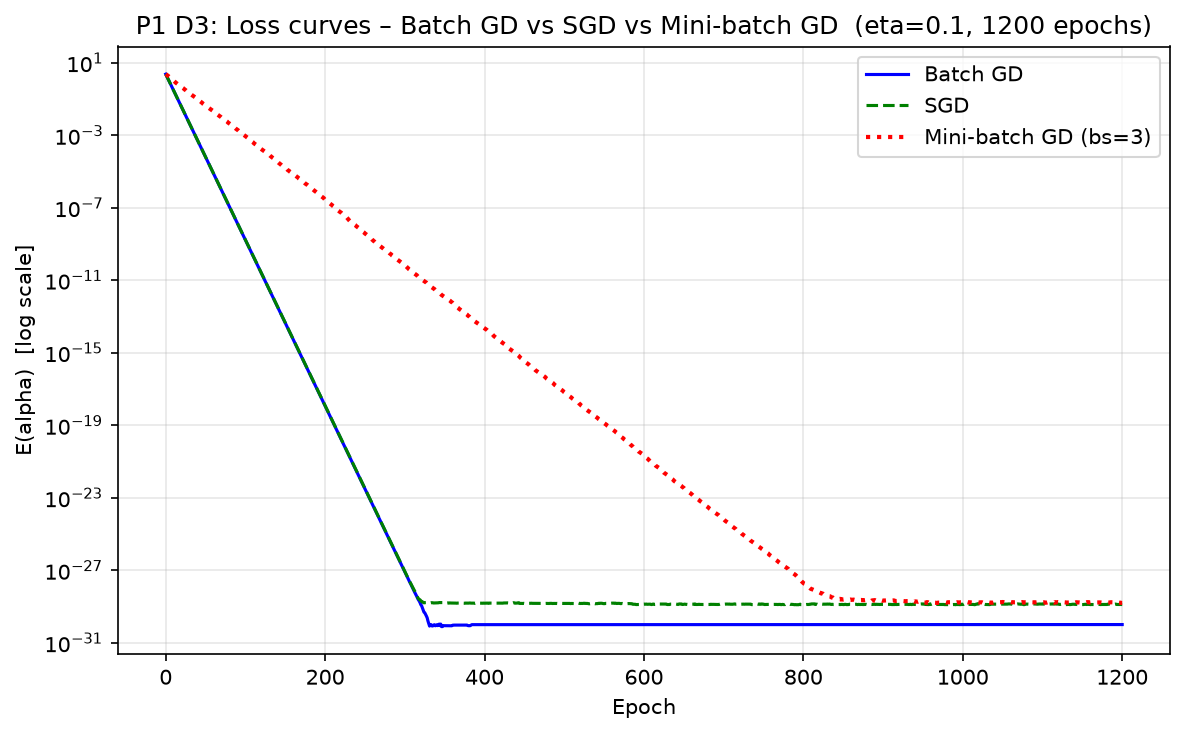
\includegraphics[width=0.88\linewidth]{images/p1_d3_loss_curves.png}
\caption{Batch GD, SGD and mini-batch GD loss curves (eta = 0.1)}
\end{figure}
\begin{table}[H]
\centering
\caption{Final error floor after convergence}
\small
\begin{tabular}{|lr|}
\toprule
Method & Final E \\
\midrule
Batch GD & 1.006972e-30 \\
SGD & 1.291692e-29 \\
Mini-batch GD & 1.562047e-29 \\
\bottomrule
\end{tabular}
\end{table}


\subsection{D4 -- Learning-Rate Study}
\begin{figure}[H]
\centering
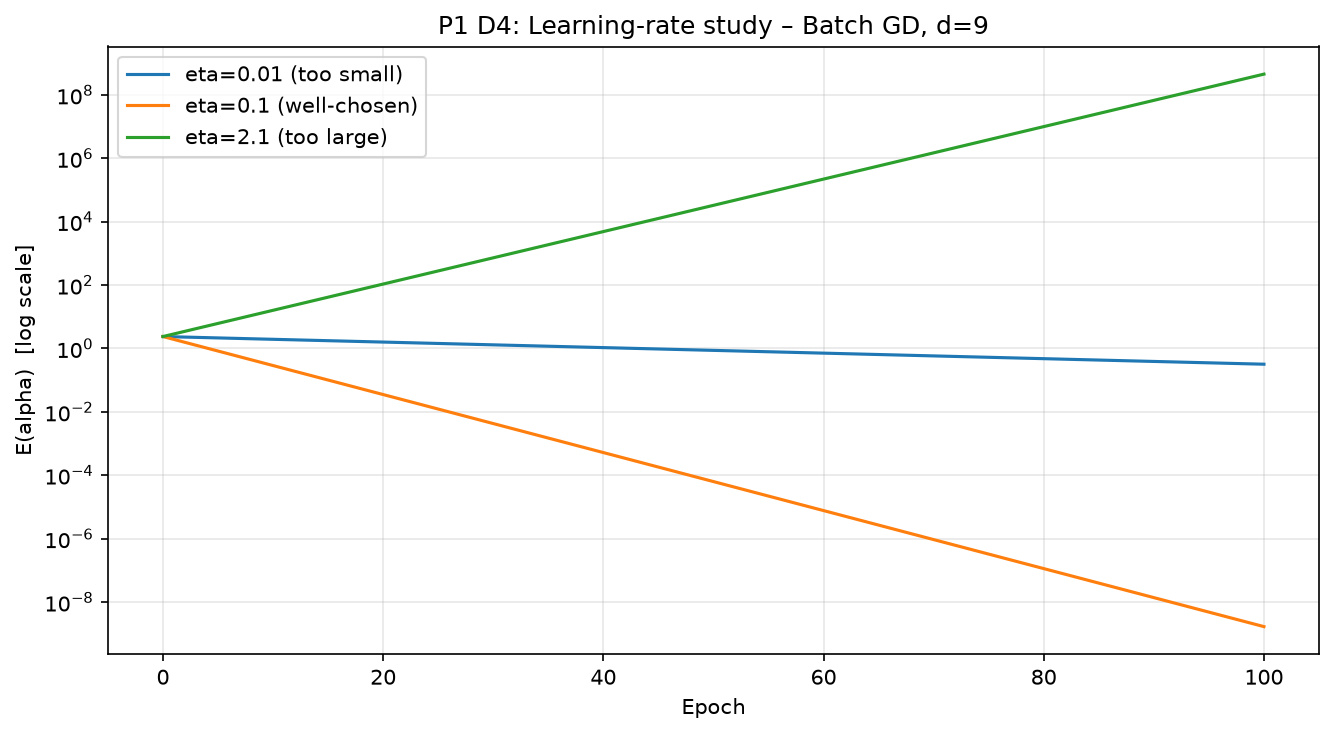
\includegraphics[width=0.88\linewidth]{images/p1_d4_lr_study.png}
\caption{Learning-rate study, 100 epochs}
\end{figure}
\begin{table}[H]
\centering
\caption{Learning-rate comparison at epoch 100}
\small
\begin{tabular}{|lr|}
\toprule
eta & Final E (epoch 100) \\
\midrule
0.01 & 3.189640e-01 \\
0.1 & 1.679595e-09 \\
2.1 & 4.521056e+08 \\
2 (special case) & 2.380690e+00 \\
\bottomrule
\end{tabular}
\end{table}

\noindent\textbf{Divergent weight vector ($\eta = 2.1$, 100 epochs):} Objective value $E = 4.521056\times 10^8$.
\begin{Verbatim}[frame=single,fontsize=\small]
w = [-2.3295e+03, -2.9307e+05,  5.6983e+06, -5.2197e+07,  2.4236e+08,
     -6.2843e+08,  9.5644e+08, -8.4896e+08,  4.0607e+08, -8.0691e+07]
\end{Verbatim}



\subsection{D5 -- Verification Against Closed Form (2000 Epochs)}
\begin{table}[H]
\centering
\caption{Verification against closed form}
\small
\begin{tabular}{|lrr|}
\toprule
Method & \textbar{}\textbar{}w\_GD - w\_cf\textbar{}\textbar{}\_2 & Relative error \\
\midrule
Batch GD & 3.178392e-06 & 2.911191e-11 \\
SGD & 3.178918e-06 & 2.911674e-11 \\
Mini-batch GD & 3.178157e-06 & 2.910976e-11 \\
\bottomrule
\end{tabular}
\end{table}

\begin{Verbatim}[frame=single,fontsize=\small]
||w_closed||_2 = 1.091784e+05
cond(R) = 1.5193e+07
\end{Verbatim}
All three variants agree with the closed form to order $10^{-11}$ relative (a few $10^{-6}$ absolute); the error is the same for all three variants and is machine-dependent round-off amplified by $\mathrm{cond}(R) \sim 1.5\times 10^7$ when recovering $w = R^{-1}\alpha$, not by the choice of GD variant.

\subsection{D6 -- Discussion}
With the QR reparametrisation Q is orthogonal, so E(alpha) has curvature 1 in every direction and each full pass over the data contracts the error by \textbar{}1 - eta\textbar{} = 0.9 (eta = 0.1); the loss curves in the figure are straight lines on the log scale for that reason. Batch GD and SGD lie on top of each other: the rows of Q are orthonormal, so each single-sample step in SGD touches one alpha-direction and one epoch updates every direction once, exactly as batch GD does. Mini-batch GD descends visibly more slowly because averaging the gradient over a batch shrinks the per-sample step, yet all three reach a round-off floor (final E 1.006972e-30, 1.291692e-29 and 1.562047e-29 respectively).

\section{P2 -- Ridge Regression as MAP}

\subsection{D1 -- Closed-Form Ridge}
Ridge weights are obtained via \texttt{np.linalg.solve} on $(\Phi^T\Phi + \lambda I) w = \Phi^T t$; resulting fits and errors are reported below.

\subsection{D2 -- Gradient-Descent Agreement and Conditioning}
\begin{figure}[htbp]
\centering
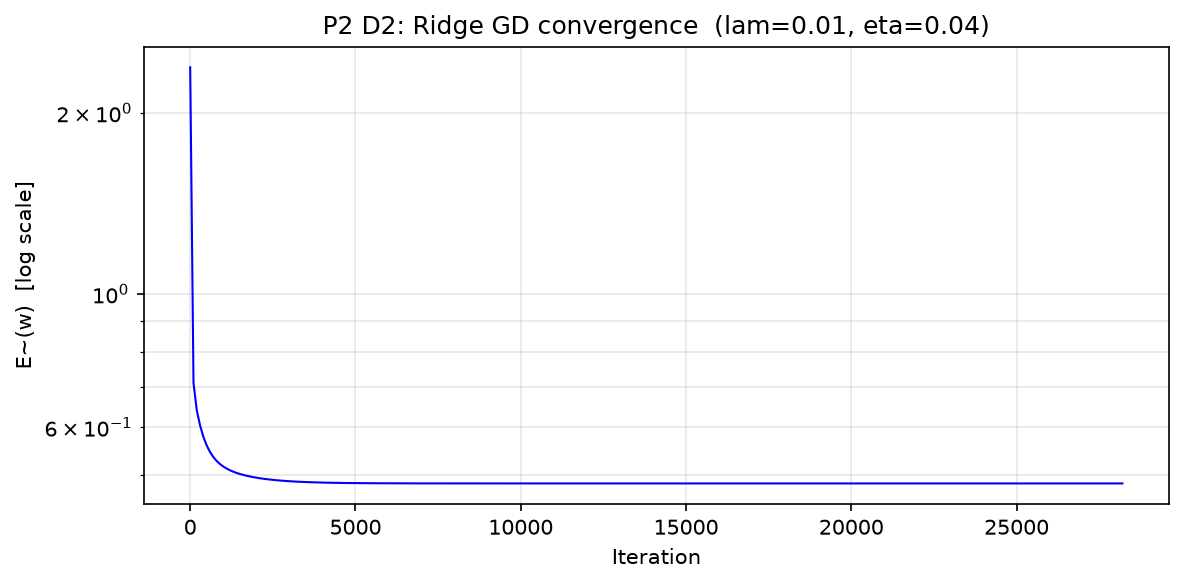
\includegraphics[width=0.88\linewidth]{images/p2_d2_gd_convergence.png}
\caption{Ridge GD loss vs iteration (lam = 0.01)}
\end{figure}
\begin{table}[htbp]
\centering
\caption{Conditioning and convergence of Ridge GD}
\small
\begin{tabularx}{0.9\textwidth}{|>{\raggedright\arraybackslash}Xr|}
\toprule
Quantity & Value \\
\midrule
cond(Phi\textasciicircum T Phi) & 2.3124e+14 \\
cond(Phi\textasciicircum T Phi + lam I), lam = 0.01 & 2.0381e+03 \\
GD iterations to converge & 28227 \\
Relative error vs closed form & 9.9968e-07 \\
\bottomrule
\end{tabularx}
\end{table}

Without the penalty the normal matrix is extremely ill-conditioned (cond = 2.3124e+14), whereas adding lam = 0.01 on the diagonal brings it down to 2.0381e+03, which is why gradient descent converges (28227 iterations, relative error 9.9968e-07).

\subsection{D3 -- RMSE Sweep and the Lambda Interval}
\begin{figure}[htbp]
\centering
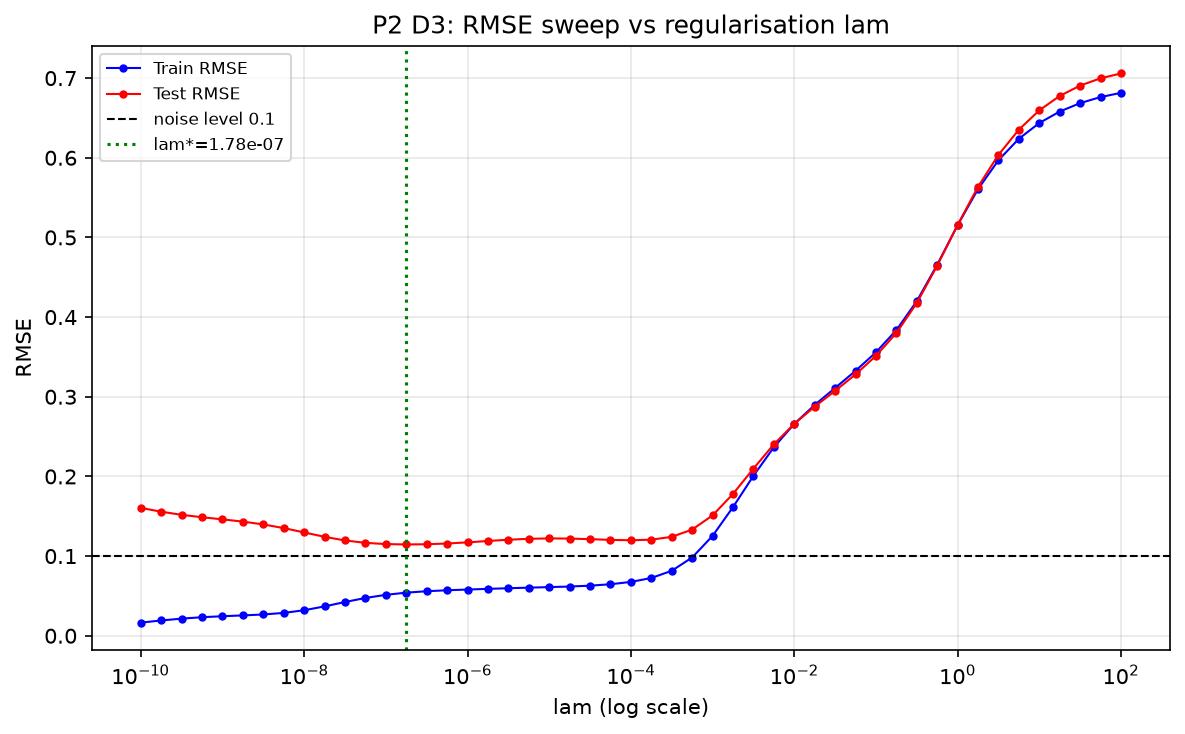
\includegraphics[width=0.88\linewidth]{images/p2_d3_rmse_sweep.png}
\caption{Train and test RMSE vs lambda}
\end{figure}
\begin{table}[htbp]
\centering
\caption{Optimal regularisation parameter}
\small
\begin{tabularx}{0.85\textwidth}{|>{\raggedright\arraybackslash}Xr|}
\toprule
Quantity & Value \\
\midrule
lam* & 1.7783e-07 \\
Test RMSE at lam* & 0.114577 \\
Interval (test RMSE within 5\% of min) & [3.1623e-08, 1.0000e-04] \\
\bottomrule
\end{tabularx}
\end{table}

The test-RMSE minimum is flat rather than sharp: every lam in [3.1623e-08, 1.0000e-04] stays within 5\% of the minimum (0.114577 at lam* = 1.7783e-07), so lam need not be tuned precisely. Below 3.1623e-08 the model overfits (train RMSE keeps falling while test RMSE rises), and above 1.0000e-04 it underfits (both RMSEs rise as the weights are shrunk too hard).

\subsection{D4 -- Fitted Curves}
\begin{figure}[htbp]
\centering
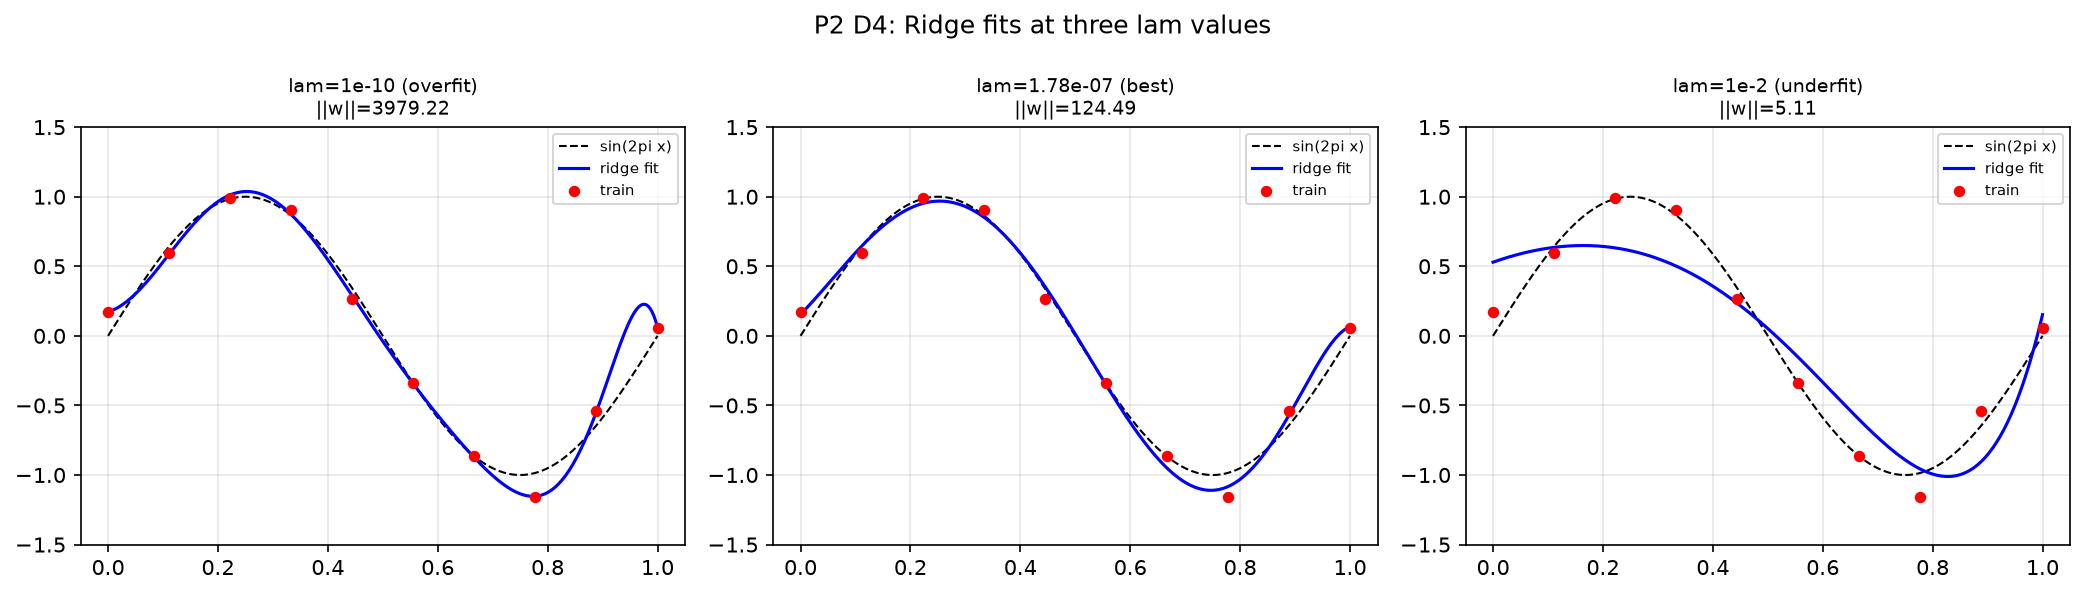
\includegraphics[width=0.88\linewidth]{images/p2_d4_fitted_curves.png}
\caption{Fitted curves at lam = 1e-10, lam* and lam = 1e-2}
\end{figure}
\begin{table}[htbp]
\centering
\caption{Weights under different regularisation regimes}
\small
\begin{tabular}{|lrr|}
\toprule
lam & Regime & \textbar{}\textbar{}w\textbar{}\textbar{}\_2 \\
\midrule
lam = 1e-10 & overfit & 3979.2246 \\
lam = 1.78e-07 & best & 124.4946 \\
lam = 1e-2 & underfit & 5.1079 \\
\bottomrule
\end{tabular}
\end{table}


\section{P3 -- Lasso via Subgradient Descent}

\subsection{D1 -- Detailed Analysis at $\lambda = 0.1$}
\begin{figure}[H]
\centering
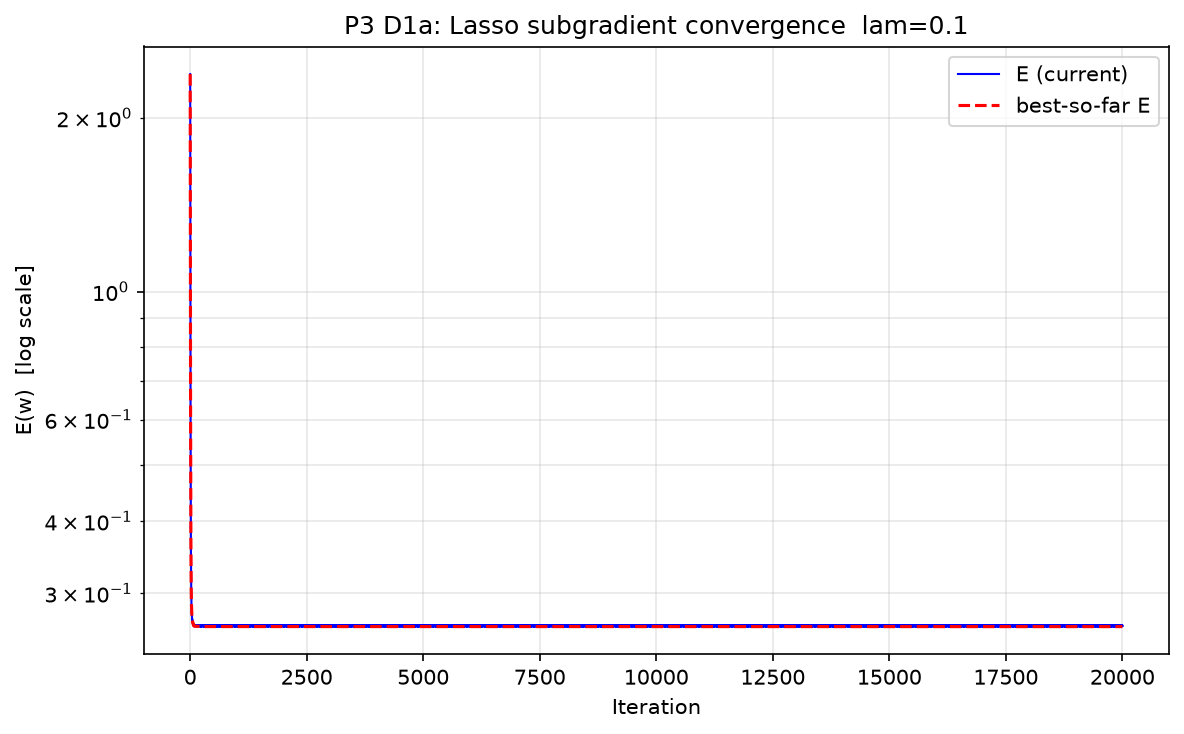
\includegraphics[width=0.88\linewidth]{images/p3_d1a_convergence.png}
\caption{Subgradient loss and best-so-far at lam = 0.1}
\end{figure}
\begin{table}[H]
\centering
\caption{Subgradient optimality and convergence metrics at lam = 0.1}
\small
\begin{tabularx}{0.95\textwidth}{|>{\raggedright\arraybackslash}Xr|}
\toprule
Quantity & Value \\
\midrule
Final E & 0.263570 \\
Best E & 0.262619 \\
E - E* & 0.001070 \\
E* (3-decimal reference) & 0.2625 \\
\textbar{}\textbar{}w - w*\textbar{}\textbar{}\_2 & 0.007636 \\
max \textbar{}Phi\_j\textasciicircum T r - lam sign(w\_j)\textbar{} (non-zero w\_j) & 1.435812e-02 \\
max \textbar{}Phi\_j\textasciicircum T r\textbar{} / lam (zero w\_j) & 0.683041 \\
Non-zero coefficient indices & [1, 2, 3, 4, 5, 7] \\
Zero coefficient indices & [0, 6, 8, 9] \\
\bottomrule
\end{tabularx}
\end{table}


\subsection{D2 -- RMSE Sweep}
\begin{figure}[H]
\centering
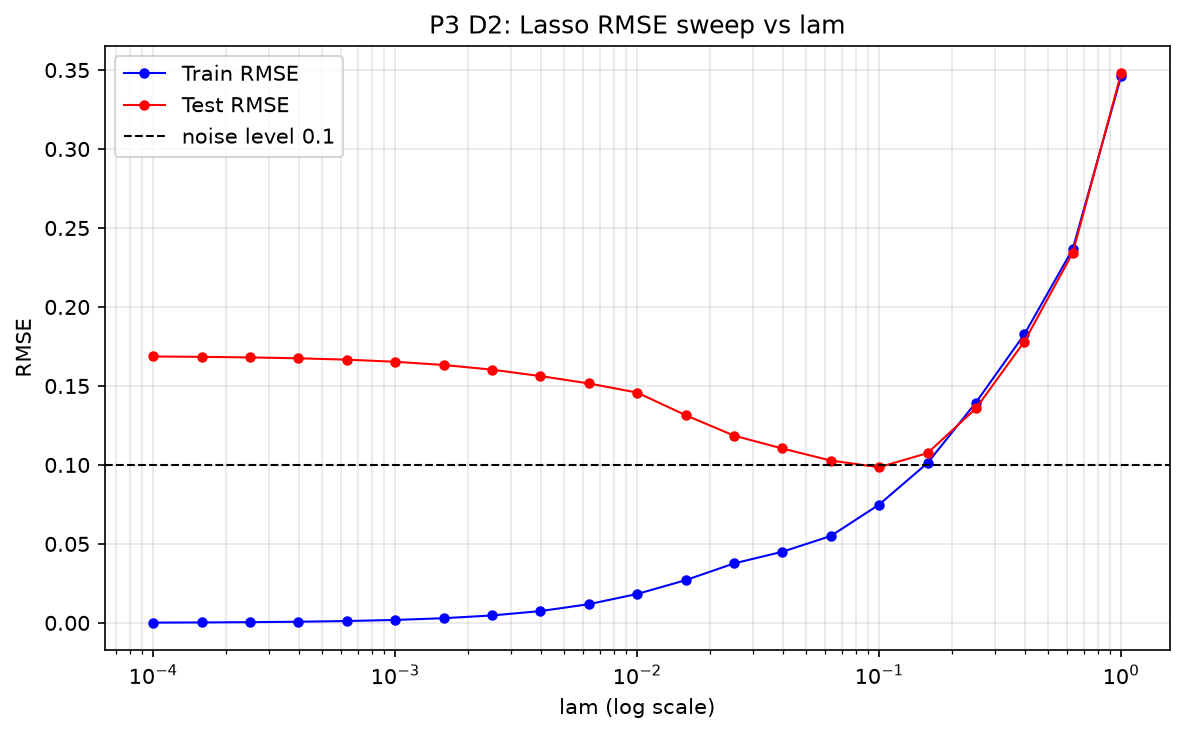
\includegraphics[width=0.88\linewidth]{images/p3_d2_rmse_sweep.png}
\caption{Lasso train and test RMSE vs lambda}
\end{figure}


\subsection{D3 -- Coefficient Path}
\begin{figure}[H]
\centering
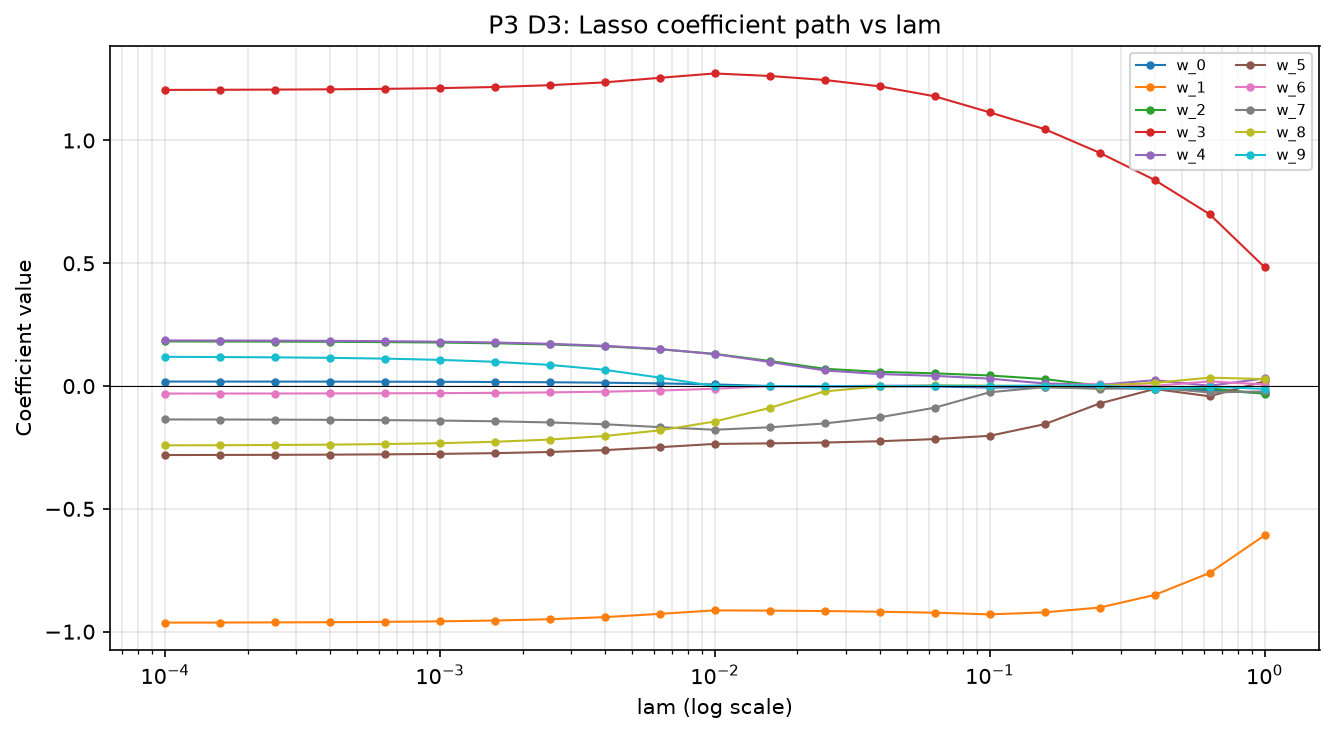
\includegraphics[width=0.88\linewidth]{images/p3_d3_coef_path.png}
\caption{Coefficient path vs lambda}
\end{figure}
\begin{table}[H]
\centering
\caption{Lasso coefficient pruning vs lambda}
\small
\begin{tabularx}{0.85\textwidth}{|r>{\raggedleft\arraybackslash}X|}
\toprule
lam & \# \textasciitilde zero coefficients (\textbar{}w\_j\textbar{} < 2*eta*lam) \\
\midrule
1.0000e-04 & 0 \\
1.5849e-04 & 0 \\
2.5119e-04 & 0 \\
3.9811e-04 & 0 \\
6.3096e-04 & 0 \\
1.0000e-03 & 0 \\
1.5849e-03 & 0 \\
2.5119e-03 & 0 \\
3.9811e-03 & 0 \\
6.3096e-03 & 0 \\
1.0000e-02 & 1 \\
1.5849e-02 & 3 \\
2.5119e-02 & 3 \\
3.9811e-02 & 4 \\
6.3096e-02 & 4 \\
1.0000e-01 & 4 \\
1.5849e-01 & 6 \\
2.5119e-01 & 7 \\
3.9811e-01 & 8 \\
6.3096e-01 & 8 \\
1.0000e+00 & 8 \\
\bottomrule
\end{tabularx}
\end{table}


\subsection{D4 -- Best Lambda}
\begin{table}[H]
\centering
\caption{Best Lasso hyperparameters}
\small
\begin{tabularx}{0.85\textwidth}{|>{\raggedright\arraybackslash}Xr|}
\toprule
Quantity & Value \\
\midrule
lam* & 1.0000e-01 \\
Test RMSE at lam* & 0.098544 \\
\# \textasciitilde zero coefficients & 4 \\
Indices & [0, 6, 8, 9] \\
\bottomrule
\end{tabularx}
\end{table}


\subsection{D5 -- Lasso vs Ridge Comparison (Legendre Basis)}
\begin{table}[H]
\centering
\caption{Lasso vs Ridge on Legendre basis}
\small
\begin{tabularx}{\textwidth}{|lrrr>{\raggedleft\arraybackslash}X|}
\toprule
Method & lam* & Test RMSE & \textbar{}\textbar{}w\textbar{}\textbar{}\_2 & \# coeffs \textbar{}w\_j\textbar{} < 0.01 \\
\midrule
Lasso & 1.0000e-01 & 0.098544 & 1.4667 & 4 \\
Ridge & 1.5849e-01 & 0.142233 & 1.4406 & 1 \\
\bottomrule
\end{tabularx}
\end{table}


\subsection{D6 -- Fitted Curves}
\begin{figure}[H]
\centering
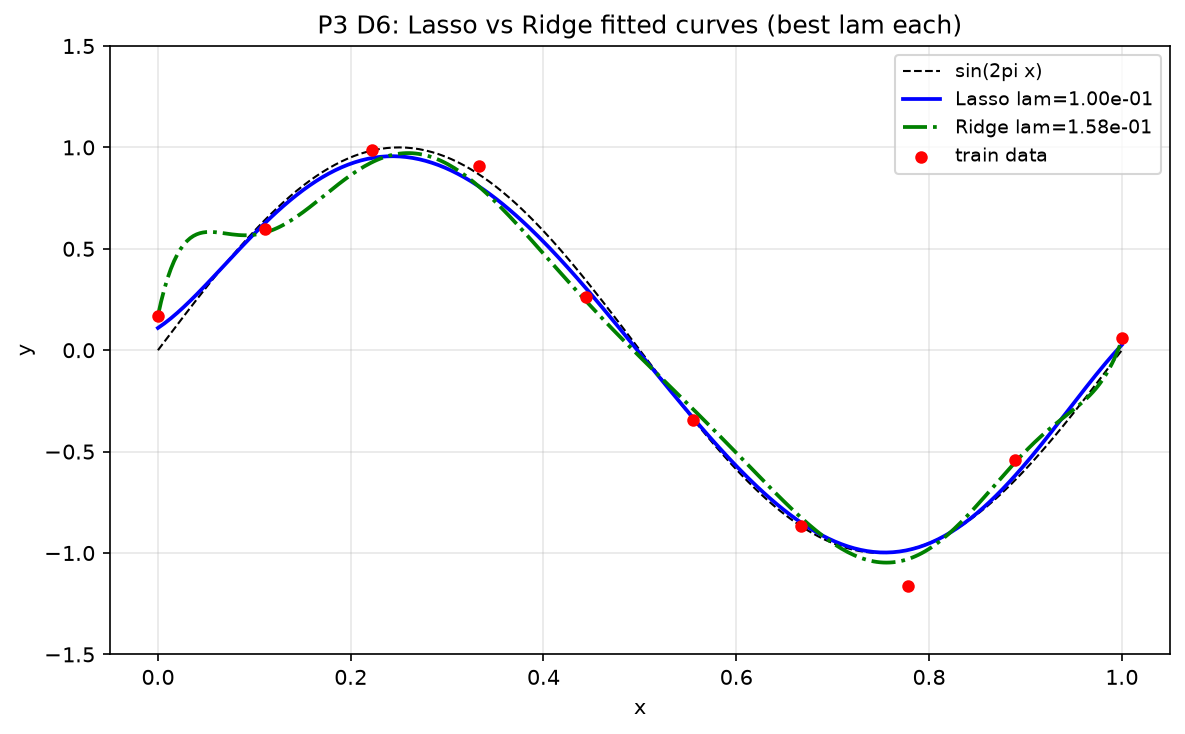
\includegraphics[width=0.88\linewidth]{images/p3_d6_fitted_curves.png}
\caption{Lasso vs Ridge at their respective best lambda}
\end{figure}


\subsection{D7 -- Discussion}
The L1 penalty yields exact zeros because a zero coefficient is optimal whenever the subgradient condition \textbar{}Phi\_j\textasciicircum T r\textbar{} <= lam holds (here max \textbar{}Phi\_j\textasciicircum T r\textbar{}/lam = 0.683041 on the zero set), and the L1 ball has corners on the axes; the L2 penalty only shrinks coefficients, which is why ridge leaves 1 coefficient(s) below 0.01 against 4 for lasso. For lam >= lam* = 1.0000e-01 the train RMSE and the test RMSE both increase as lam grows, because the extra sparsity removes model capacity that the data support and the fit moves from the noise level (0.098544 at lam*) towards underfitting.

\section{P4 -- Bayesian Linear Regression}

\subsection{D1 -- Posterior Predictive ($N = 10$)}
Hyperparameters: alpha=0.05, beta=100.0, degree=3.
\begin{figure}[htbp]
\centering
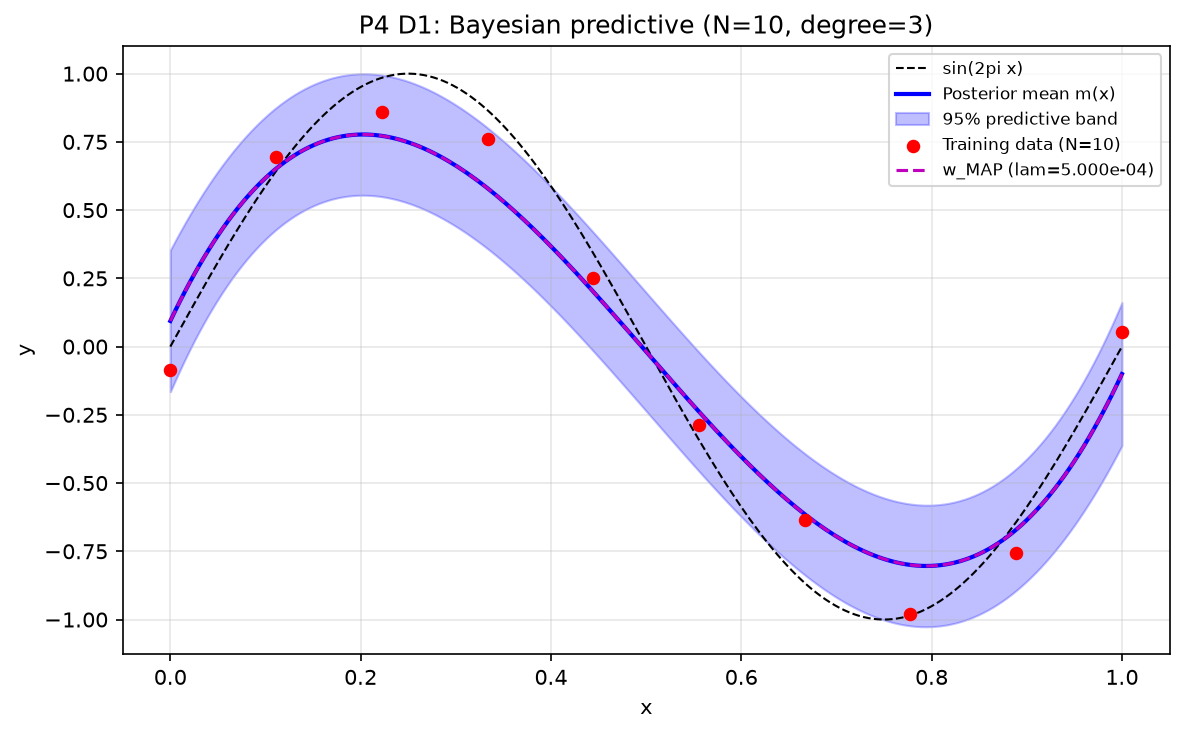
\includegraphics[width=0.88\linewidth]{images/p4_d1d2_predictive_N10.png}
\caption{Posterior mean, 95\% credible band and w\_MAP overlay (N = 10)}
\end{figure}


\subsection{D2 -- Equivalence of Posterior Mean and MAP}
\begin{Verbatim}[frame=single,fontsize=\small]
lam = alpha/beta = 5.000000e-04
||w_MAP - m_N||_2 = 1.1276e-12
\end{Verbatim}

\subsection{D3 -- Interval Width vs $N$}
\begin{figure}[htbp]
\centering
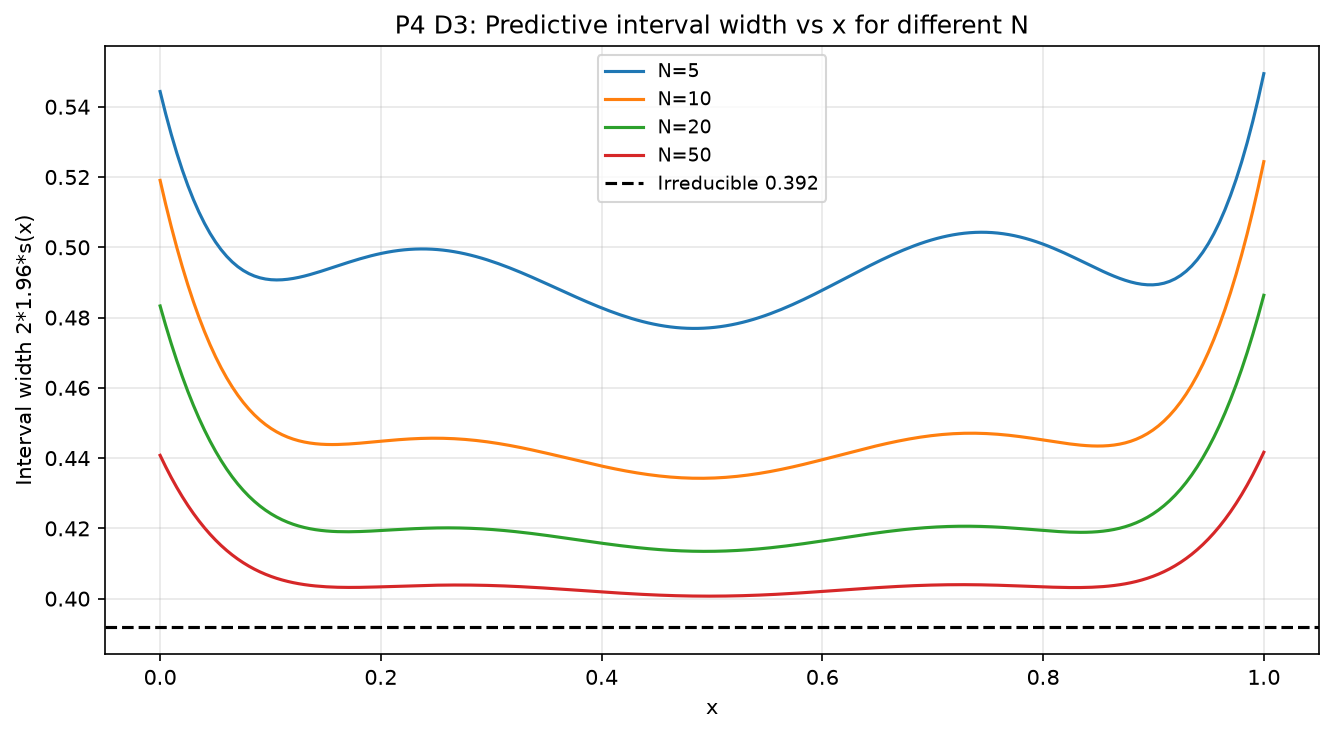
\includegraphics[width=0.88\linewidth]{images/p4_d3_interval_width.png}
\caption{Predictive interval width 2*1.96*sigma(x) for N = 5, 10, 20, 50}
\end{figure}
\begin{table}[htbp]
\centering
\caption{Predictive interval width summary}
\small
\begin{tabular}{|lrr|}
\toprule
N & Mean width & Max width \\
\midrule
5 & 0.4952 & 0.5494 \\
10 & 0.4491 & 0.5244 \\
20 & 0.4242 & 0.4863 \\
50 & 0.4064 & 0.4417 \\
\bottomrule
\end{tabular}
\end{table}

Irreducible floor: $2\times 1.96 / \sqrt{\beta} = 0.3920$.

\subsection{D4 -- Discussion}
As N grows the data term beta*Phi\textasciicircum T Phi dominates the posterior precision, so S\_N shrinks and the parameter-uncertainty part phi\textasciicircum T S\_N phi of the predictive variance falls; the mean interval width drops from 0.4952 at N=5 to 0.4064 at N=50. It cannot go below the floor 2*1.96/sqrt(beta) = 0.3920, because the noise term 1/beta in the predictive variance is irreducible however much data we collect.

\section*{Notes}
\begin{itemize}
  \item P1 solves the polynomial fit in the QR reparametrisation (Phi = QR, alpha = R w), where Q\textasciicircum T Q = I and every curvature equals 1; weights are recovered as w = R\textasciicircum -1 alpha with a linear solve.
  \item No explicit matrix inverses are used for the weights: np.linalg.lstsq (P1 closed form) and np.linalg.solve (P2, P4). Only the P4 posterior covariance, needed for the predictive variance, uses np.linalg.inv.
  \item P3 approximate-zero threshold: throughout P3 (D1, D3, D4), a coefficient is considered approximately zero when $|w_j| < 2\eta\lambda$ (the chatter amplitude of constant-step subgradient descent with $\eta = 0.05$; at $\lambda = 0.1$ in D1, this evaluates to $2(0.05)(0.1) = 0.01$). In contrast, the P3 Deliverable 5 Lasso--Ridge comparison uses the fixed threshold $|w_j| < 0.01$ to provide a standardized comparison of sparsity between Lasso and Ridge.
  \item Subgradient descent with a constant step does not converge exactly: iterates chatter around the optimum with amplitude of order eta*lam, so the final E and \textbar{}\textbar{}w - w*\textbar{}\textbar{} keep a small non-zero gap (P3 D1), and the best-so-far E is also reported.
  \item The P3 reference E* and w* are 3-decimal values from the assignment, so gaps below about 1e-3 are within their rounding.
\end{itemize}

\end{document}
